\subsection{Allgemeines}
\label{subsec:pofallgemeines}

Optische Wellenleiter verwenden Licht zur Übertragung von Informationen. Dies
ermöglicht eine schnellere Datenübertragung als mit Kupferkabeln. Glasfaserkabel
werden mittlerweile für die Verbindung von Städten und Kontinenten, aufgrund
ihrer hohen Reichweite von mehreren Kilometern und der hohen
Übertragungsleistung von bis zu 32 Gigabit/s, eingesetzt. Aber auch die
Anschließung von Gebäuden und Wohnungen mithilfe von Lichtwellenleitern ist ein
erklärtes Ziel der Telekommunikationsunternehmen. Projekte wie
\shorthandoff{"}"Fiber to the Home"\shorthandon{"} oder \shorthandoff{"}"Fiber
to the Building"\shorthandon{"} sollen Privatpersonen und Unternehmen an das
Glasfasernetz anschließen und hohe Übertragungsgeschwindigkeiten ermöglichen.
Jedoch sind Glasfaserkabel für die Verlegung in Gebäuden ungeeignet, da diese
nur durch Fachpersonal mit Spezialwerkzeug vorgenommen werden kann und relativ
teuer ist \cite{poflan}. Polymer Optische Fasern (POF) bieten sich hier als
kostengünstige Alternative an. Sie lassen sich einfach und platzsparend verlegen
(Durchmesser beträgt ca. 1 mm) und auf kurzen Distanzen (< 100 m) können
Datenraten von bis zu 40 Gigabit/s \cite{pofacgif} erreicht werden (bei
zunehmender Entfernung nimmt die Datenkapazität ab) \cite{pofacprofile}.
POF-Kabel werden nicht nur für den Anschluss an das Internet eingesetzt sondern
auch in Flugzeugen, Zügen Automobilen und Industrieanlagen.
\autoref{fig:pofgrund} zeigt die Gründe für die Verwendung in dem jeweiligen
Bereich. Wie ausschlaggebend die Kritirien sind, wird durch den zunehmenden
Radius des Kreises in der dazugehörigen Zelle angezeigt. Für fast alle Bereiche
ist die elekmagnetische Störfestigkeit, also die Resistenz gegen
elektromagnetisch Strahlung, elektrische Felder und Magnetfelder, welche den
Fluss von Elektronen beeinträchtigen, einer der Hauptgründe, da POFs für die
Verbindung der Sensorik zum Einsatz kommen und eine Störung dieser fatale Folgen
haben könnte. Bei Flugzeugen spielt das Gewicht und die Funkenbildung ebenfalls
eine große Rolle. Durch das geringe Gewicht von POF-Kabel reduziert sich der
Treibstoffverbrauch und damit die Betriebskosten. Polymer Optische Fasern
übertragen im Gegensatz zu einem Kupferkabel keine Elektronen sondern Licht und
können somit keine Funken bilden. Dadurch wird eine mögliche Gefahrenquelle
eliminiert.

\begin{figure}[h]
    \begin{center}
        \begin{minipage}[t]{\textwidth}
            \begin{center}
                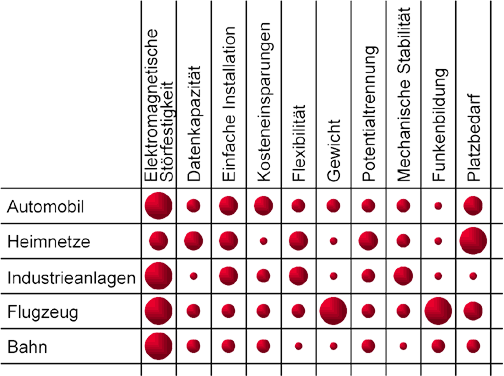
\includegraphics[height=0.2\textheight]{Bilder/Optische_Wellenleiter_Die_Polymer_Optische_Faser/Allgemeines/pofgrund.png}
                \caption[Gründe für die Verwendung von POF-Kabel \newline \url{http://www.pofac.fh-nuernberg.de/pofac/de/was_sind_pof/images/warum_pof.png}]{Gründe für die Verwendung von POF-Kabel}
                \label{fig:pofgrund}
            \end{center}
        \end{minipage}
    \end{center}
\end{figure}
